
\subsection{Validation of stage1 triggers using simulations}
Almost all of stage one trigger components, before deploying to the production firmware, were tested on GEANT4 simulated data.

\subsection{Validation of electron trigger based on ``Beam ON" data}
\label{sec:validation_random}

The ultimate validation of the trigger is done using the so called ''Random Trigger" (RT) runs.
RT runs are special runs, where event readout is initiated not by the trigger logic, but by an external random generator, that
can be tuned on the desired frequency. Most of events in RT runs will not contain any tracks, or other useful information, however,
small fraction of events will have real reconstructed particles which were reconstructed because accidentally detector's response
signal to the particle felled in the readout window that was initiated by the random generator.
In the event readout in addition to various detector signals, the trigger decisions are stored as well (see section {\color{Red} XX, somewhere above
it should be described, how trigger decisions are made, and what is the clock cycle for trig decisions }).

We want to use these accidental ``Good" events, and check whether corresponding trigger bit is set by trigger logic ({\color{Red} I assume
trigger bits will be described above}).
%%%%%%%%%%%%%%%%%%%%%%%%%%%%%%%%%%%%%%%%% F I G U R E %%%%%%%%%%%%%%%%%%%%%%%%%%%%%%%%%%%%%%%%%%
\begin{figure}[!htb]
 \centering
 \subfloat[]{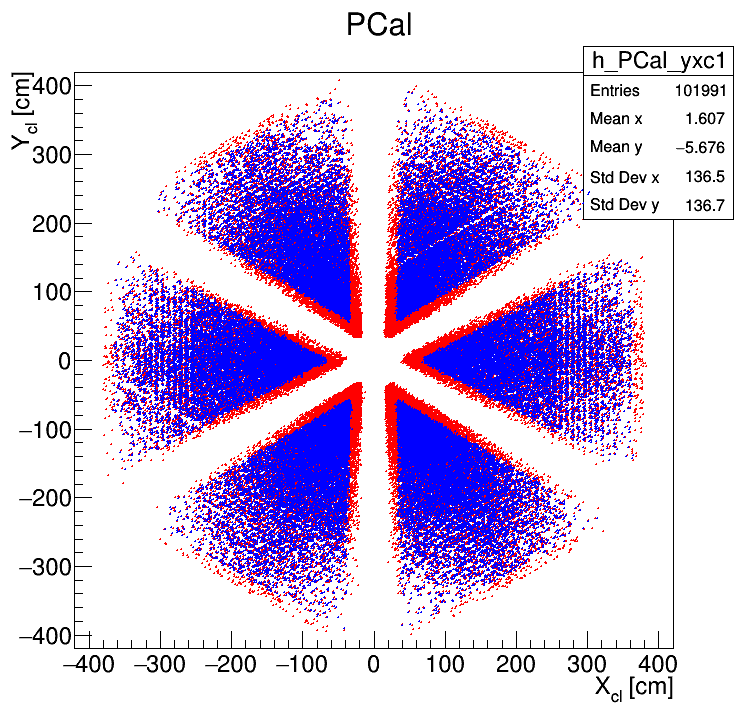
\includegraphics[width=0.24\textwidth]{img/PCal_Fiducials_4878.png}}
 \subfloat[]{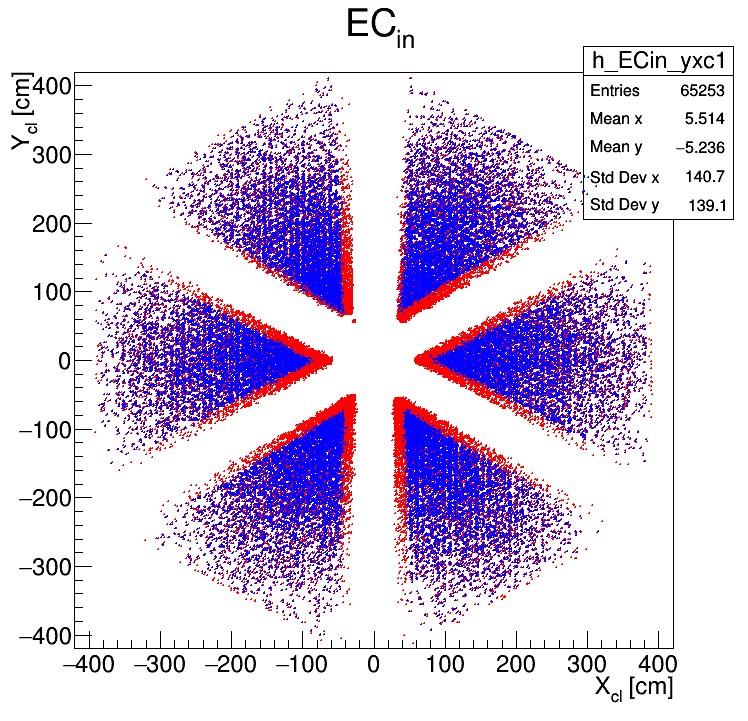
\includegraphics[width=0.24\textwidth]{img/ECin_Fiducials_4878.png}}
 \caption{Distribution of cluster coordinates of PCal (left) and EC\_{in} (right).
 scatter plot in Red shows all events, while blue scatter plot show events where cluster
 is in the fiducial region of the calorimeter (about 15 cm away from the edges).}
\end{figure}
%%%%%%%%%%%%%%%%%%%%%%%%%%%%%%%%%%%%%%%%% F I G U R E %%%%%%%%%%%%%%%%%%%%%%%%%%%%%%%%%%%%%%%%%%

The technique of the trigger validation is the following, Trigger logic is configured exactly as it will be set in experiment, but it is running in tagging mode reporting trigger decisions into data stream for every randomly generated event. After several hours of running we are collecting at least 100 million events.

Fig. ~\ref{fig:htcc_fadc1} shows typical FADC pulses for regular (not random) trigger, with pulse width below 50ns. Reconstructing and analysing data, we select events with signal in the middle of the FADCs window to make sure we do not have boundary effects when signal will be cut. Based on typical pulse shape we ignore areas below 50ns and above 150ns (Fig. ~\ref{fig:htcc_fadc2}).

\begin{figure}[hbt]
	\centering
	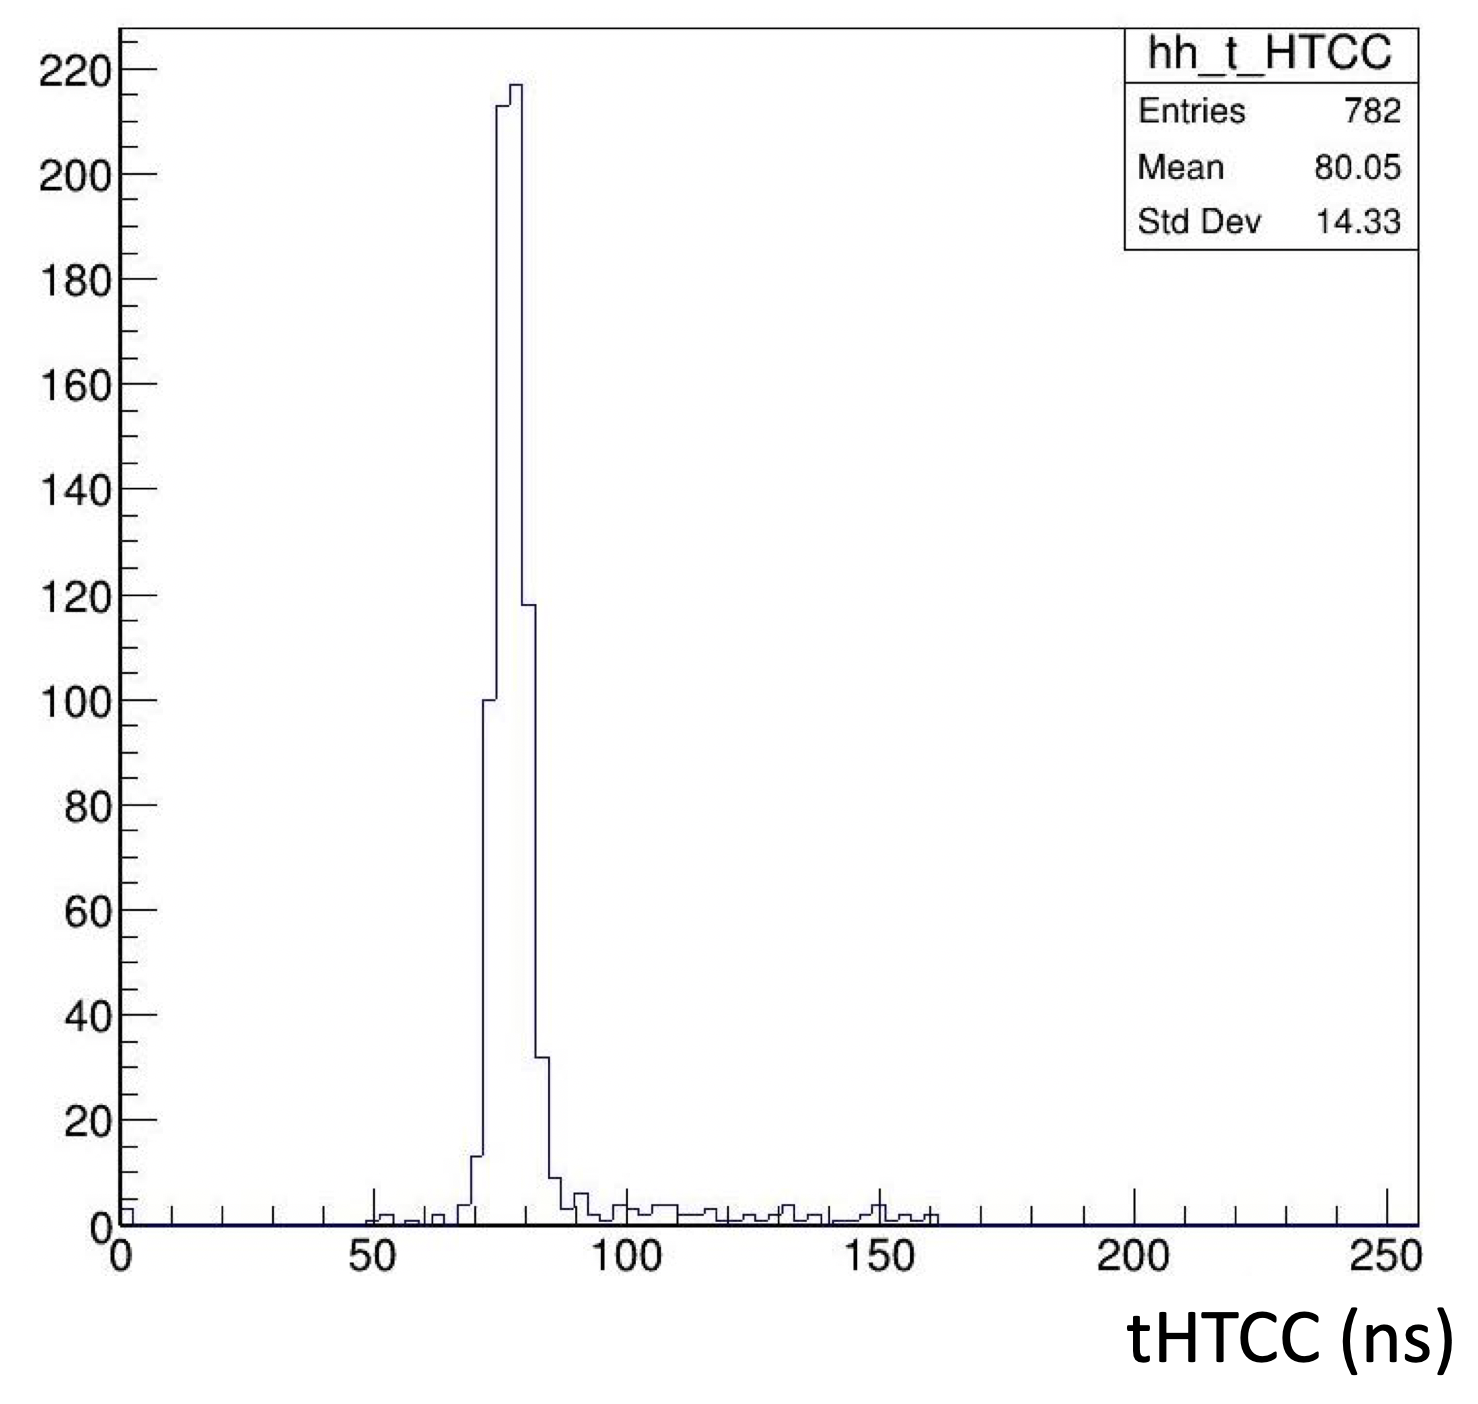
\includegraphics[width=1.0\columnwidth,keepaspectratio]{img/htcc_fadc1.png}
	\caption{HTCC FADC pulses (physics trigger)}
	\label{fig:htcc_fadc1}
\end{figure}

\begin{figure}[hbt]
	\centering
	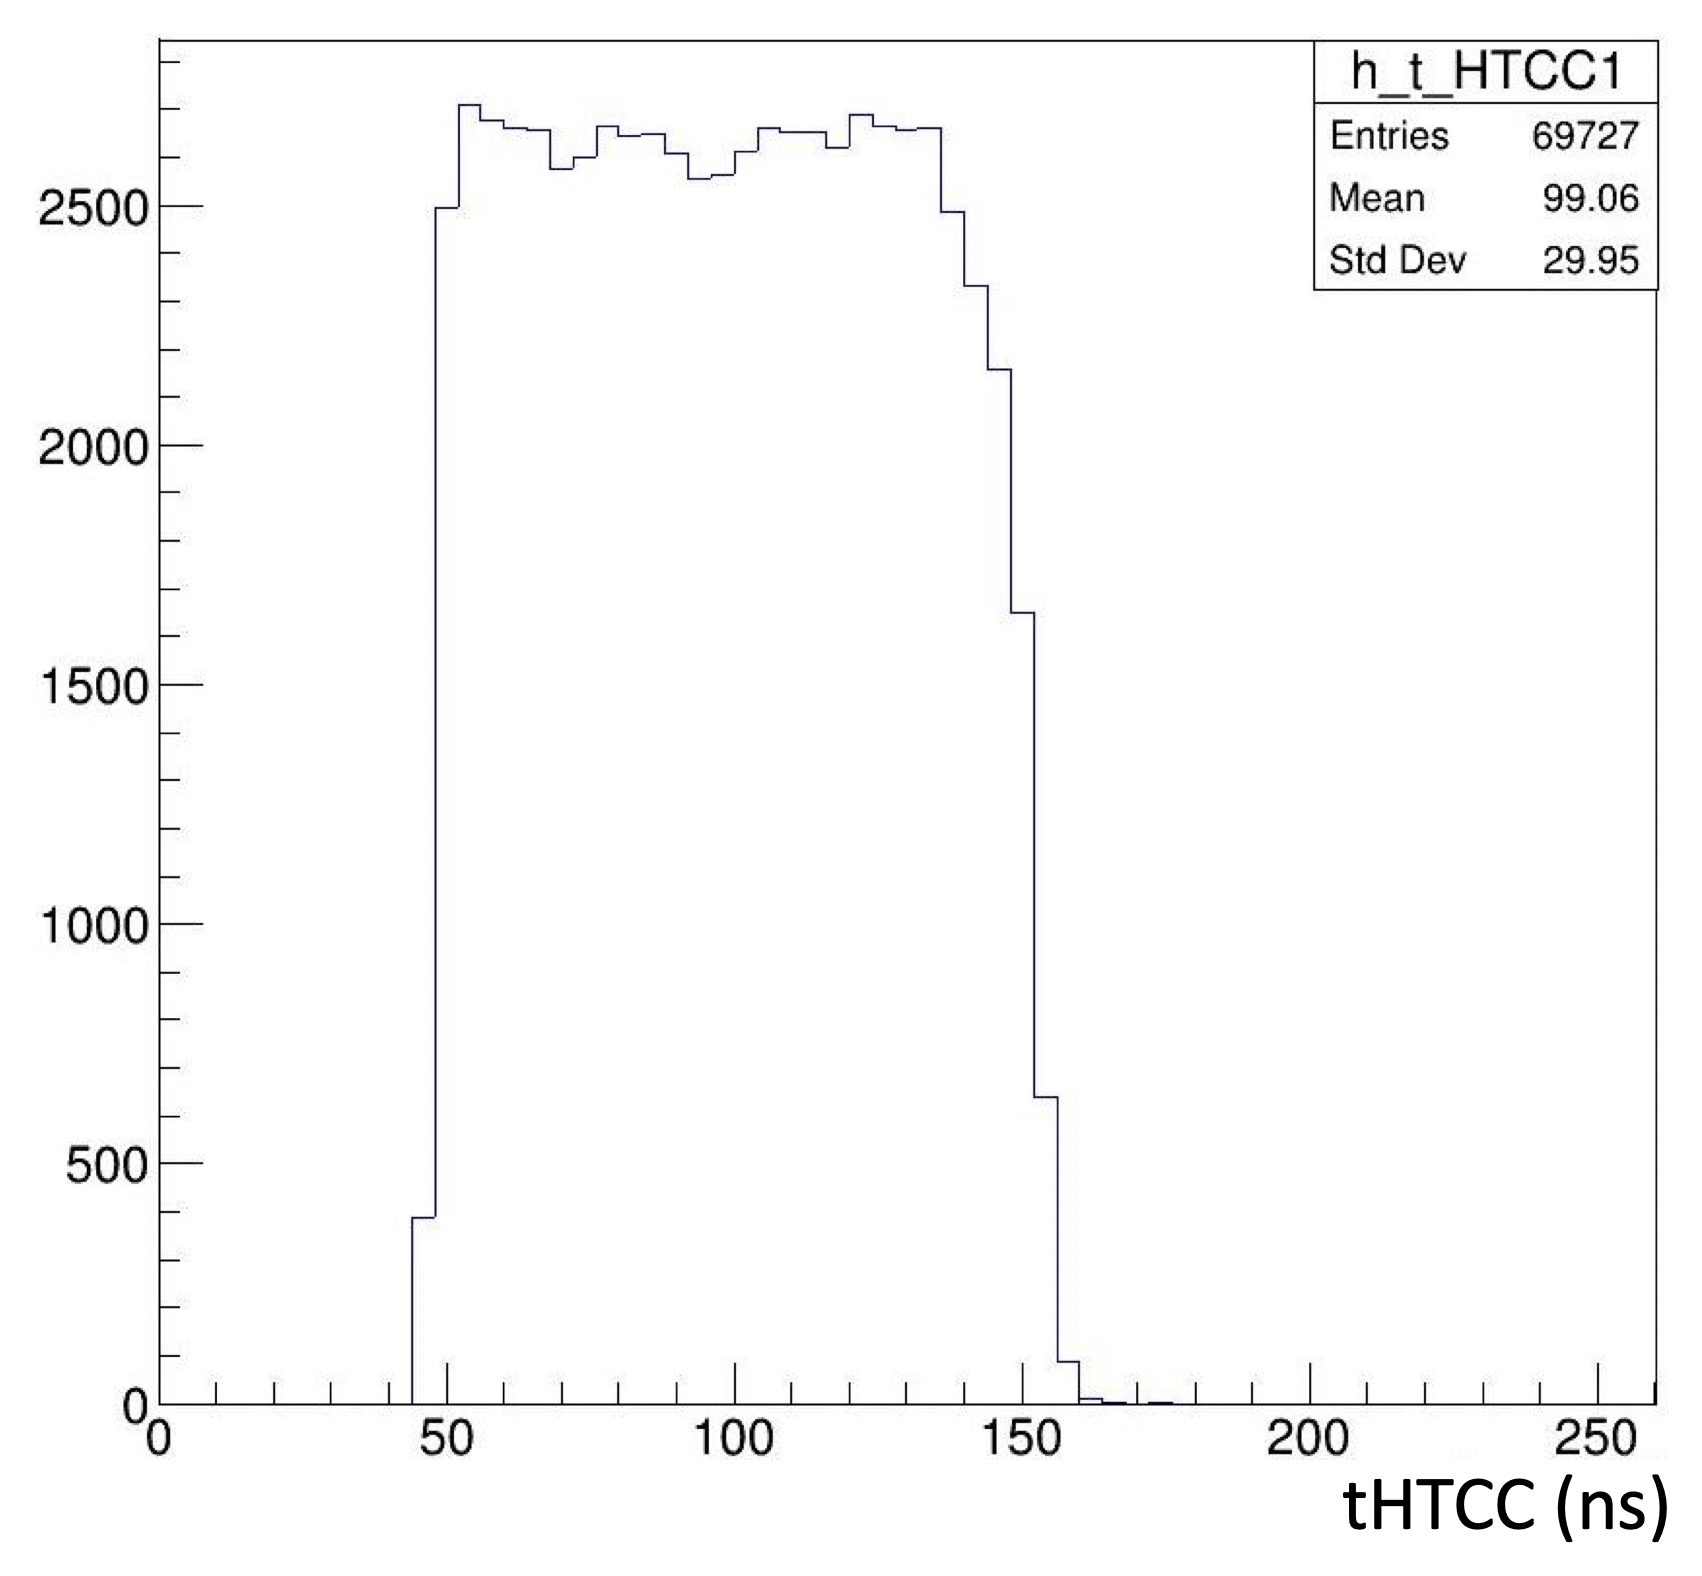
\includegraphics[width=1.0\columnwidth,keepaspectratio]{img/htcc_fadc2.png}
	\caption{HTCC FADC pulses (random trigger)}
	\label{fig:htcc_fadc2}
\end{figure}

 After data processed and events reconstructed, we will find several thousands events which accidently fell into correct trigger window. Those events will be used to obtain trigger efficiency and purity assuming that our off-line reconstruction software works correctly. It should be mentioned that working off-line reconstruction is important pre-requisite for trigger validation.
 